\documentclass[a4paper, 10pt, final]{article}
\usepackage{bonde}

\def\mytitle{Signal and Image Processing 2010}
\def\mysubtitle{Handin of mandatory excercise 5}
\def\myauthor{Ulrik Bonde}
\def\mymail{\mailto{bonde@diku.dk}}
\def\mydate{\today}

\title{\mytitle}
\subtitle{\mysubtitle}

\author{\myauthor{} - \mymail}
\date{\mydate}

\hypersetup{
colorlinks,%
citecolor=black,%
filecolor=black,%
linkcolor=black,%
urlcolor=black,%
bookmarksopen=false,
pdftitle={\mytitle{} - \mysubtitle},
pdfauthor={\myauthor}
}

\begin{document}
\maketitle

\subsection*{Question 5.1}
The following will answer \citep[Excercise 11.6, p. 329]{jahne-digital}.

\paragraph{1)}
I will show that it is not possible to improve the signal-to-noise ratio
for an arbitrary single wave number. The SNR is defined as
\begin{equation}
    SNR = \frac{\sigma^2_N}{\sigma^2_S}
\end{equation}
i.e. the variance of the noise divided by the variance of the signal. By
\citep[Eq. (4.38)]{jahne-digital} we are given a measure for the
variance of a signal convolved with a filter $\mathcal{H}$:
\begin{equation}
    \mathbf{\sigma'} = \sigma^2(\mathcal{H} \star
    \mathcal{H})~ ~\laplace~ ~
    \mathbf{\hat{\sigma}'} = \hat{\sigma}(k)|\hat{\mathcal{H}}|^2
\end{equation}
Using this we write up the SNR for the filtered signal.
\begin{align}
    SNR' & =
    \frac{\sigma^2_N(\mathcal{H}\star\mathcal{H})}{\sigma^2_S(\mathcal{H}\star\mathcal{H})}
    ~ ~\laplace~
    ~\frac{\hat{\sigma}^2_S(k)|\hat{\mathcal{H}}(k)|^2}{\hat{\sigma}^2_N(k)|\hat{\mathcal{H}}(k)|^2}\\
    & = \frac{\sigma^2_N}{\sigma^2_S}
    ~ ~\laplace~
    ~\frac{\hat{\sigma}^2_S(k)}{\hat{\sigma}^2_N(k)}\\
    SNR' & = SNR
\end{align}
The signal to noise ratio is the same in a filtered signal as in the
original signal. Intuitively, if we have a signal and we can divide it
into a signal and noise part, when we filter both parts with the same
filter, then the ratio between the signal and noise will be the same.

\paragraph{2)}
Now, if we assume that we have white noise, but the actual signal only
exist in half of the maximum wave numbers, then we can actually improve
the SNR. The explanation is pretty straight forward. We know in which
frequencies the actual signal is and we know that we have some high
frequency noise. Some of the noise does not interfere with the original
signal, thus we can just remove the frequencies where we \emph{only}
have noise. Fig. \ref{box_filter_model} illustrate this in a two
dimensional signal. The noise is removed by using a box filter.

\begin{figure}[!h]
    \centering
    \subfloat[Original]{\label{org}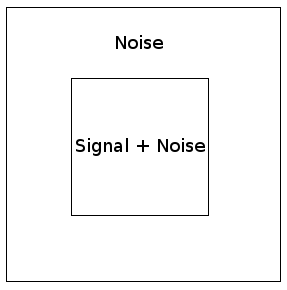
\includegraphics[angle=0,width=0.3\textwidth]{images/spectrum_im_noise}}\hspace{1em}
    \subfloat[Box filter]{\label{box_filter}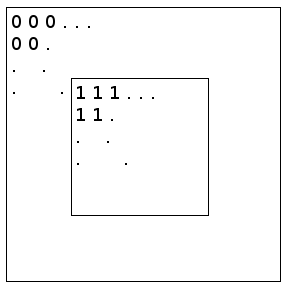
\includegraphics[angle=0,width=0.3\textwidth]{images/filter_box}}\hspace{1em}
    \subfloat[Filtered signal]{\label{filtered}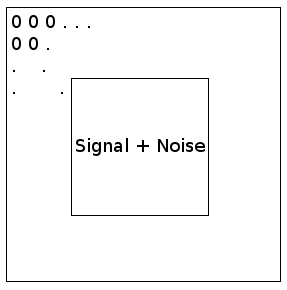
\includegraphics[angle=0,width=0.3\textwidth]{images/filtered_im}}\\
    \caption[]{Frequency representation of the original signal where the
    actual signal is limited to the middle of the power spectrum. Using
    a box filter we can remove the unwanted frequencies, i.e. the noise.
    In the resulting signal these frequencies have been zeroed out.}
    \label{box_filter_model}
\end{figure}

Because we have \emph{only} removed noise and not manipulated the actual
signal we have improved the SNR.

Using an alternative definition for SNR saying
\begin{equation}
    SNR = \frac{\mu}{\sigma_N}
\end{equation}
and realize that $\sigma_N$ is constant (because it is white noise) it
is clear how the SNR is improved. When we remove the unwanted
frequencies the value of $\mu$ is decreased, thus the SNR is improved.

\subsection*{Question 5.2}
\paragraph{1}

\begin{figure}[!h]
    \centering
    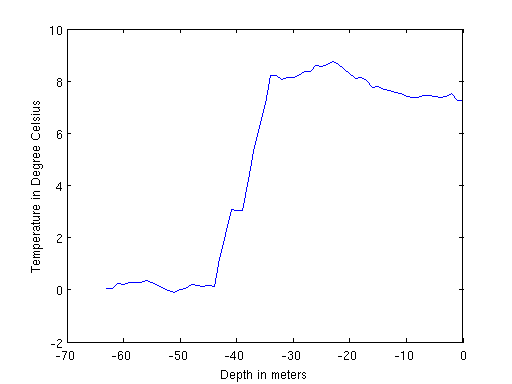
\includegraphics[angle=0,width=0.7\textwidth]{images/org_signal}
    \caption[]{Original signal}
    \label{org_signal}
\end{figure}

For finding the border between two temperature zones I have implemented
a simple edge detector. Edges are found using the second derivative of
the signal. Zero crossings in the second derivative correspond to the
point in the original signal where a given gradient have the steepest
slope. A measure for this slope is found in the same point in the first
derivative. Using a threshold value small fluctuations in the signal is
ruled out.

The original signal --- shown in Fig. \ref{org_signal} --- is noisy,
hence we find derivatives in a smoothed signal. For smoothing I use a
Gaussian kernel with $\sigma = 5/4$.  Before smoothing the signal is
expanded using replication of border values. The smoothed signal is
shown in Fig. \ref{blur_signal}.

\begin{figure}[!h]
    \centering
    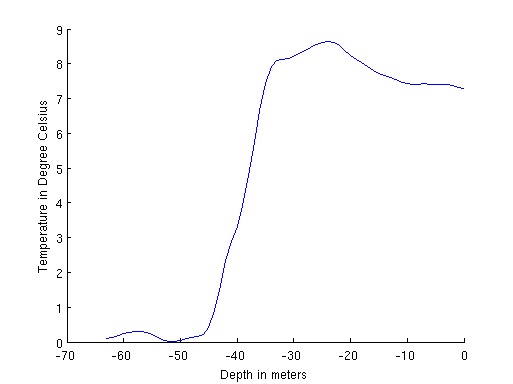
\includegraphics[angle=0,width=0.7\textwidth]{images/blur_signal}
    \caption[]{Smoothed signal. Convolution of expanded signal with a
    Gaussian kernel with $\sigma = 5/4$.}
    \label{blur_signal}
\end{figure}

Now we find the first and second derivative of the signal. The first
derivative is found using the backward difference from \citep[Eq.
(12.29)]{jahne-digital}. The second derivative is found using
\citep[Eq. (12.44)]{jahne-digital}, i.e. the backward difference of the
forward difference. The derivatives for the smoothed signal is shown in
Fig. \ref{derivatives}.

\begin{figure}[!h]
    \centering
    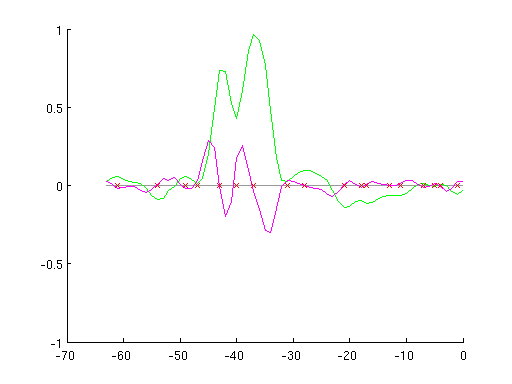
\includegraphics[angle=0,width=0.7\textwidth]{images/derivatives}
    \caption[]{Green: First order derivative. Magenta: Second order
    derivative. Red crosses: Zero crossings in the second derivative.}
    \label{derivatives}
\end{figure}

Now we find the zero crossings in the second derivative indicating a
slope in the original image. At the position of a zero crossing we look
up the value of the first derivative. If this value is above a certain
threshold we keep the value, otherwise the it is set to zero and later
removed. In this manner we can find the border between two temperature
zones in the signal. The found edge is shown in Fig.
\ref{signal_org_blur_edge}.

\begin{figure}[!h]
    \centering
    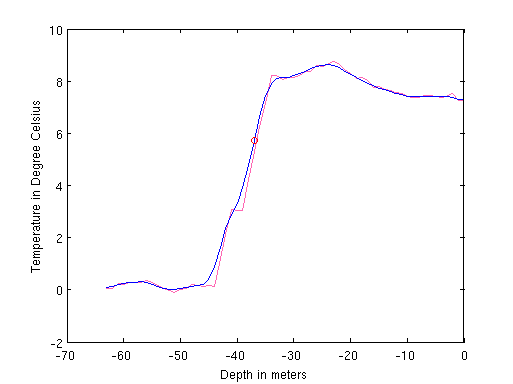
\includegraphics[angle=0,width=0.7\textwidth]{images/signal_org_blur_edge}
    \caption[]{Blue: Smoothed signal. Light red: Original signal. Red
    circle: Found edge. The edge is found at -37 meters where the
    gradient has the steepest slope.}
    \label{signal_org_blur_edge}
\end{figure}

Because the second derivative is used we do not find the start and end
points of the gradient, but rather the middle of the gradient. It is
interesting to note that we can find the start of the gradient by
locating the global maximum of the second derivative. The opposite is
not true, i.e. we can not find the end point of the gradient by finding
the global minimum.

The main methods for finding the border are included in the appendix.

\paragraph{2}
We now want to apply adaptive filtering to the signal. This allows us to
use a variable filter size for filtering certain areas with a broader
filter. Specifically we want to filter coarsely at near-constant
segments, while large changes are kept intact.

Again we use the second derivative as it gives an indication of how the
original signal changes. Reviewing Fig. \ref{derivatives} we see that at
the locations just before and after the large gradient, the second
derivative has relatively small values. Thus, when the second derivative
is small we want to use a larger filter. When the values are big, we
want a smaller filter.

Smoothing is now done in the spatial domain using a $1 \times 7$
Gaussian kernel. $\sigma$ is set by the reciprocal value of the second
derivative and adjusted by a factor $f$ as shown in eq. \eqref{sigma_val}.
\begin{equation}
    \sigma(x) = \frac{1}{|S''(x)|}f
    \label{sigma_val}
\end{equation}
The actual implementation is included in the appendix as the method
\texttt{AdaptiveFilter()}. The implementation is naive and extremely
inefficient. For each value in the final signal we convolve the entire
original signal with a new $\sigma$-value.

%%%%%%%%%%%%%%%%%%%%%%%%%%%%%%%%%%%%%%%%%%%%%%%%%%%%%%%%%%%%%%%%%%%%
% Formal stuff

\bibliographystyle{abbrvnat}
\bibliography{bibliography}
%\addcontentsline{toc}{chapter}{Litteratur}

\appendix
\lstset{language=Matlab, basicstyle=\scriptsize,
    showstringspaces=false, numbers=left, stepnumber=1,
    numberstyle=\tiny, frame=none}
\section{Source code}

\subsection{BackwardDiff.m}
\lstinputlisting{../src/BackwardDiff.m}

\subsection{ForwardDiff.m}
\lstinputlisting{../src/ForwardDiff.m}

\subsection{SymmetricDiff.m}
\lstinputlisting{../src/SymmetricDiff.m}

\subsection{EdgeDetect.m}
\lstinputlisting{../src/EdgeDetect.m}

\subsection{AdaptiveFilter.m}
\lstinputlisting{../src/AdaptiveFilter.m}

\end{document}

% vim: set tw=72 spell spelllang=en:
